\section{Binarni dijagrami odlu\v{c}ivanja}
\label{sec:BDD}

Binarni dijagrami odlu\v{c}ivanja (engl. \emph{Binary Decision Diagrams}, u daljem tekstu \emph{BDD}) su unapredjenje binarnih drveta odlu\v{c}ivanja. Prvo unapredjenje je uklanjanje redundantnih grana u drvetu. Na primer, posmatrajmo funkciju $\wedge$ definisanu u poglavlju \ref{sec:BinarnaDrvetaOdlucivanja}. U niskom pod-drvetu obe grane koje polaze od promenljive $x_{2}$ vode ka vrednosti $0$, stoga nije potrebno ispitivati vrednost promenljive $x_{2}$ \footnote{tzv. \emph{lenjo izra\v{c}unavanje}}. Ovakvom redukcijom se dobija drvo na slici \ref{diag:BDDAnd}.

\begin{figure}[H]
    \centering
    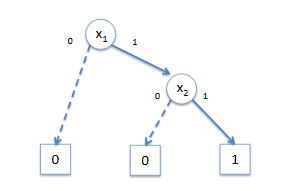
\includegraphics[scale=0.8]{slike/BDD_And.PNG}
    \caption{BDD za funkciju $\wedge$}
    \label{diag:BDDAnd}
\end{figure}

Drugo unapredjenje je dozvoljavanje deljenja identi\v{c}nih pod-drveta. Ponovo, kako bi \v{c}italac bolje razumeo \v{s}ta ovo zapravo zna\v{c}i, dajemo primer. Posmatrajmo funkciju koja ima povratnu vrednost $1$ ukoliko postoji neparan broj ulaznih promenljivih sa vredno\v{s}\'c{}u $1$, a $0$ ina\v{c}e. \v{S}tavi\v{s}e, pretpostavimo da imamo \v{c}etiri ulazne promenljive $x_{1}$, $x_{2}$, $x_{3}$ i $x_{4}$. Binarno drvo odlu\v{c}ivanja za ovakvu funkciju bi imalo 15 ($2^4 - 1$) unutra\v{s}njih \v{c}vorova i 16 ($2^4$) listova. Medjutim, BDD za ovu funkciju ima samo 7 unutra\v{s}njih \v{c}vorova i samo dva lista (slika \ref{diag:BDDParity}).

\begin{figure}[H]
    \centering
    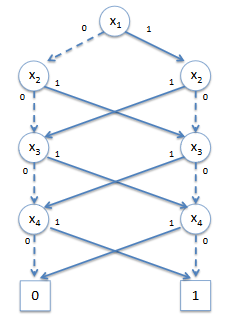
\includegraphics[scale=0.8]{slike/BDD_Parity.PNG}
    \caption{BDD za funkciju parnosti \v{c}etiri argumenta}
    \label{diag:BDDParity}
\end{figure}

U najgorem slu\v{c}aju, BDD \'c{}e biti eksponencijalno veliki u odnosu na ulaz, mada u praksi je to retko slu\v{c}aj. Takodje, konstantne funkcije se mogu predstaviti samo jednim \v{c}vorom, bez obzira na broj ulaznih promenljivih.
